\paragraph{Coordinate Noise.}
To evaluate robustness to GPS imprecision, we apply Gaussian noise to coordinates with $\sigma \in \{0, 10, 50, 100, 500, 1000\}$m, representing conditions from precise GPS to coarse IP geolocation. Each noise level contains approximately 567 samples (16.7\%).

\begin{figure}[htbp]
\centering
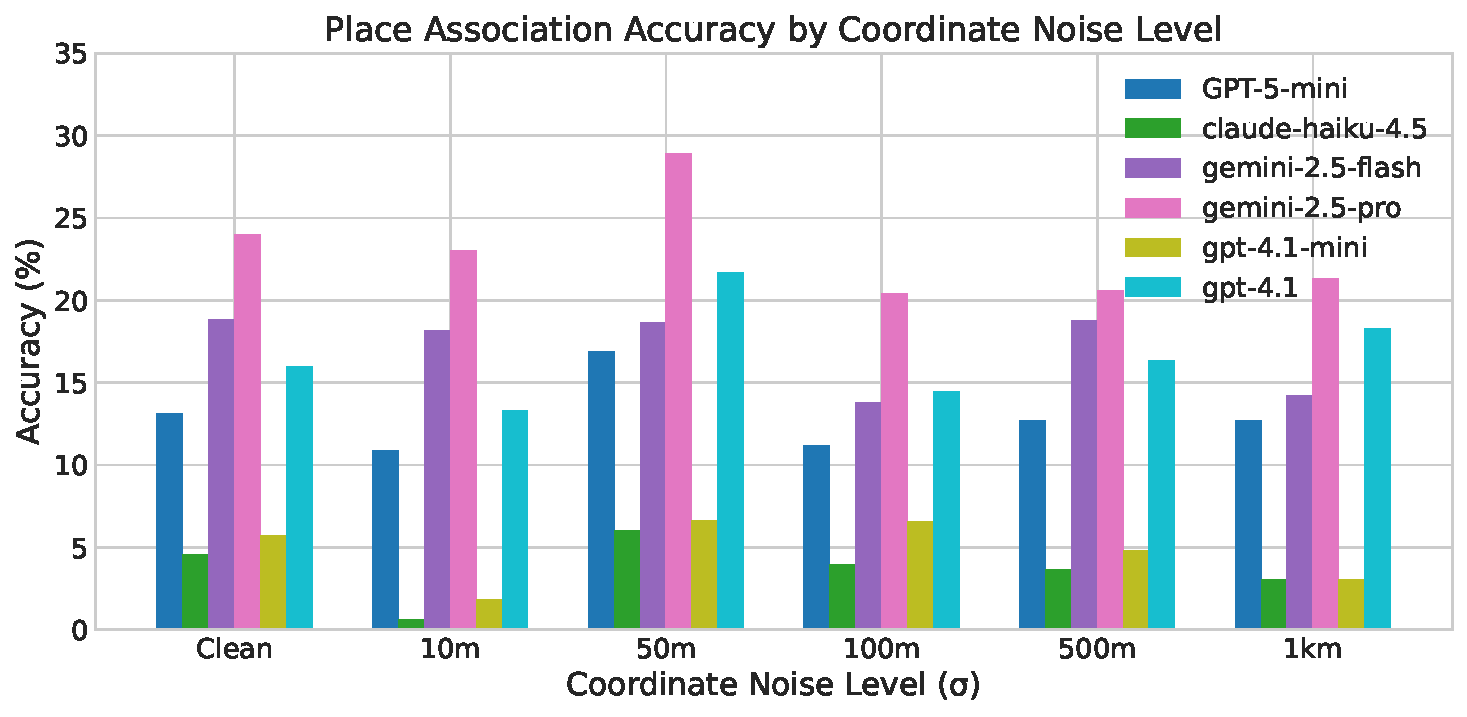
\includegraphics[width=\columnwidth]{figures/place_association_noise.pdf}
\caption{Place association accuracy by coordinate noise level. Performance remains uniformly low across all noise levels, indicating that coordinate imprecision is not the primary challenge.}
\label{fig:place_assoc_noise}
\end{figure}

\begin{table}[htbp]
\centering
\caption{Place association accuracy (\%) by noise level and granularity. City = exact match; Country = city correct OR country mentioned in response.}
\label{tab:place_assoc_noise_results}
\small
\begin{tabular}{l|cc|cc}
\toprule
& \multicolumn{2}{c|}{\textbf{City Level}} & \multicolumn{2}{c}{\textbf{Country Level}} \\
\textbf{Model} & \textbf{Clean} & \textbf{$\Delta$} & \textbf{Clean} & \textbf{$\Delta$} \\
\midrule
Gemini-2.5-Pro & 22.4 & \textcolor{gray}{+0.7} & 26.5 & \textcolor{gray}{+0.1} \\
Gemini-2.5-Flash & 17.6 & \textcolor{gray}{$-$0.6} & 21.8 & \textcolor{gray}{$-$1.2} \\
GPT-4.1 & 18.2 & \textcolor{gray}{$-$1.5} & 21.2 & \textcolor{gray}{$-$1.8} \\
GPT-5.1 & 12.9 & \textcolor{gray}{+0.0} & 16.5 & \textcolor{gray}{$-$0.8} \\
Mistral-Large & 13.5 & \textcolor{gray}{$-$2.9} & 18.2 & \textcolor{gray}{$-$3.6} \\
Claude-Haiku-4.5 & 5.3 & \textcolor{gray}{$-$1.7} & 10.6 & \textcolor{gray}{$-$2.8} \\
Qwen3-235B & 4.7 & \textcolor{gray}{$-$1.9} & 9.4 & \textcolor{gray}{$-$2.3} \\
\midrule
\textit{Mean (all 14)} & \textit{8.3} & \textit{$-$1.0} & \textit{12.6} & \textit{$-$1.9} \\
\bottomrule
\end{tabular}
\end{table}

\paragraph{Finding.}
As shown in Table~\ref{tab:place_assoc_noise_results}, model accuracy does not degrade with increasing coordinate noise at either granularity level. At city level, mean accuracy drops only 1.0\% from clean to noisy conditions (r=0.05). At country level, the degradation is similarly minimal at 1.9\% (r=$-$0.08). Even with 1km noise---far exceeding typical GPS error---performance remains essentially unchanged. Error analysis reveals that 73\% of incorrect predictions miss the country entirely, while only 5\% identify the correct country but wrong city. This noise robustness suggests that models genuinely understand the GPS coordinate system rather than memorizing specific coordinate-location pairs---if memorized, small perturbations would cause significant accuracy drops. The primary challenge is not coordinate imprecision, but the models' lack of geographic database knowledge to map positions to place names.
